\documentclass[a4paper,12pt]{article}

\usepackage{mathtext}
\usepackage[T2A]{fontenc}
\usepackage[utf8]{inputenc}
\usepackage[russian]{babel}
\usepackage{multirow}
\usepackage{slashbox}
\usepackage{makecell}
\usepackage{graphicx}
\usepackage{physics}
\usepackage{amstext}
\usepackage{caption}
\usepackage{subcaption}
\usepackage{cmap}
\usepackage{float}


\title{Лабораторная работа 4}
\author{Калашников Михаил, Б03-205}
\date{}


\begin{document}

\maketitle{Числа с плавающей точкой (C)}

\begin{enumerate}

\setcounter{enumi}{0}

\item Напишем вставку, которая путем побитовых сдвигов будет вывоводить представление числа в памяти. Возможно, есть более простой способ получить представление, о котором я не знаю.

\begin{figure}[H]
  \centering
  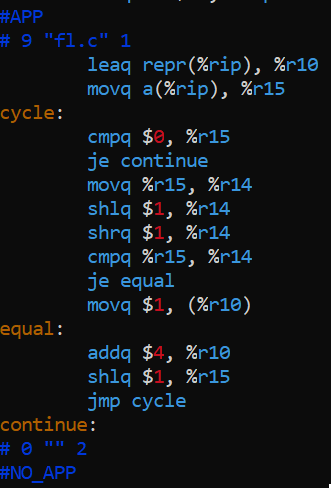
\includegraphics[width=0.6\linewidth]{images/asm4_1.png}
  \caption{}
\end{figure}

Получим представления целых чисел. Видно, что отрицательное число является дополнительным кодом положительного.

\begin{figure}[H]
  \centering
  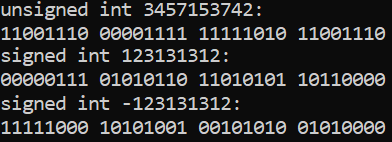
\includegraphics[width=0.6\linewidth]{images/asm4_2.png}
  \caption{}
\end{figure}

\item Выведем на экран представление float и double.

\begin{figure}[H]
  \centering
  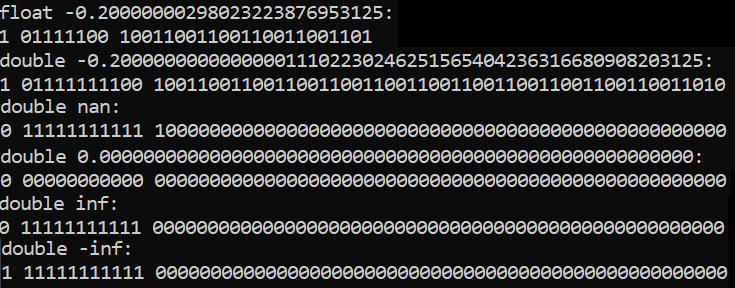
\includegraphics[width=1\linewidth]{images/asm4_3.png}
  \caption{}
\end{figure}

\item Для переполнения мантиссы достаточно присвоить дробь, которая является бесконечной в двоичной системе счисления. Это было сделано в предыдущем пункте со значением -0.2. Можно увидеть, что в памяти хранится значение, отличающееся от заданного.

\item Неассоциативность арифметических операций:

\begin{figure}[H]
  \centering
  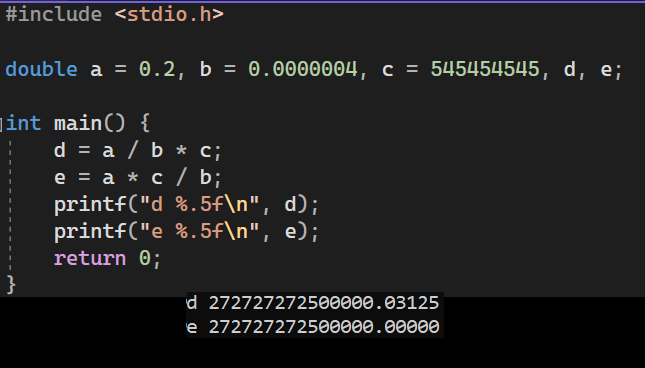
\includegraphics[width=1\linewidth]{images/asm4_4.png}
  \caption{}
\end{figure}

\item Денормализованные числа на моем процессоре работают по умолчанию и все числа с нулевой экспонентой считаются денормализованными. С помощью побитового OR можно найти минимальные значения денормализованных чисел.

\begin{figure}[H]
  \centering
  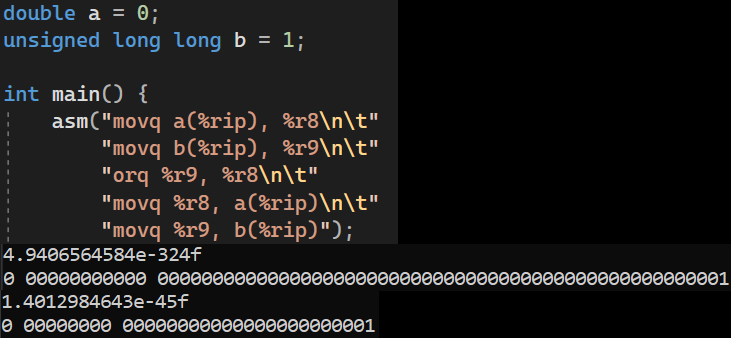
\includegraphics[width=1\linewidth]{images/asm4_5.png}
  \caption{}
\end{figure}

Выключим денормализованные числа с помощью флагов DAZ (все денормалы, которые пытаются присвоиться к даблам будут обнуляться) и FTZ (все денормалы, полученные в ходе арифметических операций будут обнуляться). Продемонстирурем эффект антипереполнения: полученный денормал обнулился.

\begin{figure}[H]
  \centering
  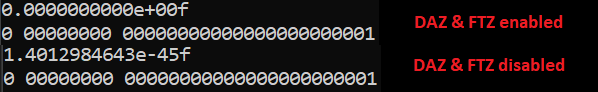
\includegraphics[width=1\linewidth]{images/asm4_6.png}
  \caption{}
\end{figure}

\item При включении флагов работа с даблами незначительно ускоряется.

\begin{figure}[H]
  \centering
  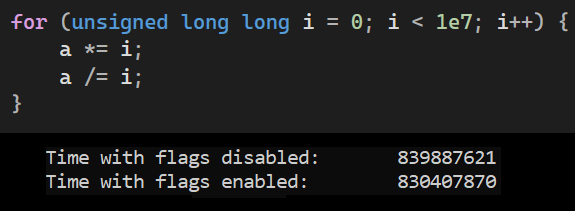
\includegraphics[width=1\linewidth]{images/asm4_7.png}
  \caption{}
\end{figure}

\item Ниже представлен график зависимости относительной ошибки от номера орбиты при численном решении задачи двух тел методом Ньютона.

\begin{figure}[H]
  \centering
  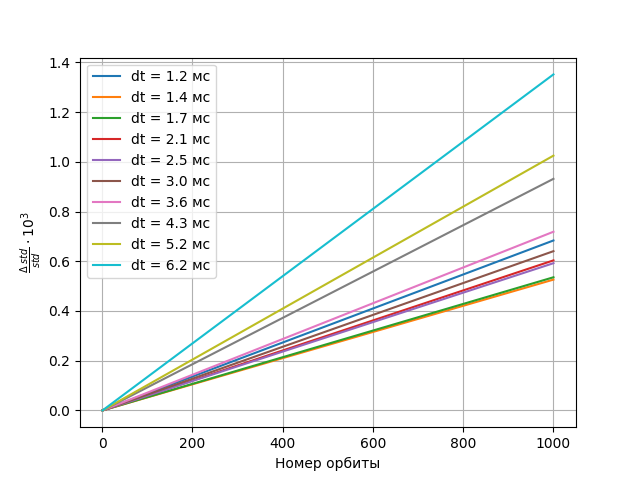
\includegraphics[width=1\linewidth]{images/asm4_8.png}
  \caption{}
\end{figure}

\end{enumerate}

\end{document}